% Options for packages loaded elsewhere
\PassOptionsToPackage{unicode}{hyperref}
\PassOptionsToPackage{hyphens}{url}
%
\documentclass[
]{ctexart}
\usepackage{amsmath,amssymb}
\usepackage{iftex}
\ifPDFTeX
  \usepackage[T1]{fontenc}
  \usepackage[utf8]{inputenc}
  \usepackage{textcomp} % provide euro and other symbols
\else % if luatex or xetex
  \usepackage{unicode-math} % this also loads fontspec
  \defaultfontfeatures{Scale=MatchLowercase}
  \defaultfontfeatures[\rmfamily]{Ligatures=TeX,Scale=1}
\fi
\usepackage{lmodern}
\ifPDFTeX\else
  % xetex/luatex font selection
\fi
% Use upquote if available, for straight quotes in verbatim environments
\IfFileExists{upquote.sty}{\usepackage{upquote}}{}
\IfFileExists{microtype.sty}{% use microtype if available
  \usepackage[]{microtype}
  \UseMicrotypeSet[protrusion]{basicmath} % disable protrusion for tt fonts
}{}
\makeatletter
\@ifundefined{KOMAClassName}{% if non-KOMA class
  \IfFileExists{parskip.sty}{%
    \usepackage{parskip}
  }{% else
    \setlength{\parindent}{0pt}
    \setlength{\parskip}{6pt plus 2pt minus 1pt}}
}{% if KOMA class
  \KOMAoptions{parskip=half}}
\makeatother
\usepackage{xcolor}
\usepackage[left=2.5cm,right=2cm,top=3cm,bottom=2.5cm]{geometry}
\usepackage{color}
\usepackage{fancyvrb}
\newcommand{\VerbBar}{|}
\newcommand{\VERB}{\Verb[commandchars=\\\{\}]}
\DefineVerbatimEnvironment{Highlighting}{Verbatim}{commandchars=\\\{\}}
% Add ',fontsize=\small' for more characters per line
\usepackage{framed}
\definecolor{shadecolor}{RGB}{248,248,248}
\newenvironment{Shaded}{\begin{snugshade}}{\end{snugshade}}
\newcommand{\AlertTok}[1]{\textcolor[rgb]{0.94,0.16,0.16}{#1}}
\newcommand{\AnnotationTok}[1]{\textcolor[rgb]{0.56,0.35,0.01}{\textbf{\textit{#1}}}}
\newcommand{\AttributeTok}[1]{\textcolor[rgb]{0.13,0.29,0.53}{#1}}
\newcommand{\BaseNTok}[1]{\textcolor[rgb]{0.00,0.00,0.81}{#1}}
\newcommand{\BuiltInTok}[1]{#1}
\newcommand{\CharTok}[1]{\textcolor[rgb]{0.31,0.60,0.02}{#1}}
\newcommand{\CommentTok}[1]{\textcolor[rgb]{0.56,0.35,0.01}{\textit{#1}}}
\newcommand{\CommentVarTok}[1]{\textcolor[rgb]{0.56,0.35,0.01}{\textbf{\textit{#1}}}}
\newcommand{\ConstantTok}[1]{\textcolor[rgb]{0.56,0.35,0.01}{#1}}
\newcommand{\ControlFlowTok}[1]{\textcolor[rgb]{0.13,0.29,0.53}{\textbf{#1}}}
\newcommand{\DataTypeTok}[1]{\textcolor[rgb]{0.13,0.29,0.53}{#1}}
\newcommand{\DecValTok}[1]{\textcolor[rgb]{0.00,0.00,0.81}{#1}}
\newcommand{\DocumentationTok}[1]{\textcolor[rgb]{0.56,0.35,0.01}{\textbf{\textit{#1}}}}
\newcommand{\ErrorTok}[1]{\textcolor[rgb]{0.64,0.00,0.00}{\textbf{#1}}}
\newcommand{\ExtensionTok}[1]{#1}
\newcommand{\FloatTok}[1]{\textcolor[rgb]{0.00,0.00,0.81}{#1}}
\newcommand{\FunctionTok}[1]{\textcolor[rgb]{0.13,0.29,0.53}{\textbf{#1}}}
\newcommand{\ImportTok}[1]{#1}
\newcommand{\InformationTok}[1]{\textcolor[rgb]{0.56,0.35,0.01}{\textbf{\textit{#1}}}}
\newcommand{\KeywordTok}[1]{\textcolor[rgb]{0.13,0.29,0.53}{\textbf{#1}}}
\newcommand{\NormalTok}[1]{#1}
\newcommand{\OperatorTok}[1]{\textcolor[rgb]{0.81,0.36,0.00}{\textbf{#1}}}
\newcommand{\OtherTok}[1]{\textcolor[rgb]{0.56,0.35,0.01}{#1}}
\newcommand{\PreprocessorTok}[1]{\textcolor[rgb]{0.56,0.35,0.01}{\textit{#1}}}
\newcommand{\RegionMarkerTok}[1]{#1}
\newcommand{\SpecialCharTok}[1]{\textcolor[rgb]{0.81,0.36,0.00}{\textbf{#1}}}
\newcommand{\SpecialStringTok}[1]{\textcolor[rgb]{0.31,0.60,0.02}{#1}}
\newcommand{\StringTok}[1]{\textcolor[rgb]{0.31,0.60,0.02}{#1}}
\newcommand{\VariableTok}[1]{\textcolor[rgb]{0.00,0.00,0.00}{#1}}
\newcommand{\VerbatimStringTok}[1]{\textcolor[rgb]{0.31,0.60,0.02}{#1}}
\newcommand{\WarningTok}[1]{\textcolor[rgb]{0.56,0.35,0.01}{\textbf{\textit{#1}}}}
\usepackage{graphicx}
\makeatletter
\def\maxwidth{\ifdim\Gin@nat@width>\linewidth\linewidth\else\Gin@nat@width\fi}
\def\maxheight{\ifdim\Gin@nat@height>\textheight\textheight\else\Gin@nat@height\fi}
\makeatother
% Scale images if necessary, so that they will not overflow the page
% margins by default, and it is still possible to overwrite the defaults
% using explicit options in \includegraphics[width, height, ...]{}
\setkeys{Gin}{width=\maxwidth,height=\maxheight,keepaspectratio}
% Set default figure placement to htbp
\makeatletter
\def\fps@figure{htbp}
\makeatother
\setlength{\emergencystretch}{3em} % prevent overfull lines
\providecommand{\tightlist}{%
  \setlength{\itemsep}{0pt}\setlength{\parskip}{0pt}}
\setcounter{secnumdepth}{5}
\ifLuaTeX
  \usepackage{selnolig}  % disable illegal ligatures
\fi
\IfFileExists{bookmark.sty}{\usepackage{bookmark}}{\usepackage{hyperref}}
\IfFileExists{xurl.sty}{\usepackage{xurl}}{} % add URL line breaks if available
\urlstyle{same}
\hypersetup{
  pdftitle={统计(机器)学习第5次作业报告},
  pdfauthor={林子开 21307110161},
  hidelinks,
  pdfcreator={LaTeX via pandoc}}

\title{统计(机器)学习第5次作业报告}
\author{林子开 21307110161}
\date{}

\begin{document}
\maketitle

{
\setcounter{tocdepth}{2}
\tableofcontents
}
\hypertarget{ux7b2cux4e00ux9898ux57faux4e8eux6734ux7d20ux8d1dux53f6ux65afux7684ux5206ux7c7bux5668}{%
\section{第一题:基于朴素贝叶斯的分类器}\label{ux7b2cux4e00ux9898ux57faux4e8eux6734ux7d20ux8d1dux53f6ux65afux7684ux5206ux7c7bux5668}}

导入数据:

\begin{Shaded}
\begin{Highlighting}[]
\FunctionTok{library}\NormalTok{(readr)}
\NormalTok{data }\OtherTok{\textless{}{-}} \FunctionTok{read\_table}\NormalTok{(}\StringTok{"D:/大三上学习资料/统计(机器)学习/hw5/第一题数据.txt"}\NormalTok{, }\AttributeTok{col\_names =} \ConstantTok{FALSE}\NormalTok{)}

\NormalTok{data }\OtherTok{=} \FunctionTok{as.matrix}\NormalTok{(data)}
\NormalTok{data }\OtherTok{=} \FunctionTok{t}\NormalTok{(data)}
\FunctionTok{colnames}\NormalTok{(data) }\OtherTok{=} \FunctionTok{c}\NormalTok{(}\StringTok{\textquotesingle{}X1\textquotesingle{}}\NormalTok{,}\StringTok{\textquotesingle{}X2\textquotesingle{}}\NormalTok{,}\StringTok{\textquotesingle{}Y\textquotesingle{}}\NormalTok{)}

\NormalTok{X1 }\OtherTok{=} \FunctionTok{as.numeric}\NormalTok{(data[,}\DecValTok{1}\NormalTok{])}
\NormalTok{X2 }\OtherTok{=}\NormalTok{ data[,}\DecValTok{2}\NormalTok{]}
\NormalTok{Y }\OtherTok{=} \FunctionTok{as.numeric}\NormalTok{(data[,}\DecValTok{3}\NormalTok{])}
\end{Highlighting}
\end{Shaded}

\hypertarget{ux57faux4e8eux6781ux5927ux4f3cux7136ux4f30ux8ba1}{%
\subsection{基于极大似然估计}\label{ux57faux4e8eux6781ux5927ux4f3cux7136ux4f30ux8ba1}}

计算先验概率的极大似然估计

\begin{Shaded}
\begin{Highlighting}[]
\NormalTok{PY }\OtherTok{=} \FunctionTok{table}\NormalTok{(Y)}\SpecialCharTok{/}\FunctionTok{length}\NormalTok{(Y)}
\FunctionTok{print}\NormalTok{(PY)}
\end{Highlighting}
\end{Shaded}

\begin{verbatim}
## Y
##        -1         1 
## 0.3333333 0.6666667
\end{verbatim}

即\(P(Y=-1)=0.333,\, P(Y=1)=0.667\)。

计算条件概率的\textbf{极大似然估计}如下:

\begin{Shaded}
\begin{Highlighting}[]
\DocumentationTok{\#\# X1的条件概率的MLE}
\NormalTok{PX1.cond }\OtherTok{=} \FunctionTok{matrix}\NormalTok{(}\FunctionTok{rep}\NormalTok{(}\DecValTok{0}\NormalTok{,}\DecValTok{2}\SpecialCharTok{*}\DecValTok{3}\NormalTok{),}\AttributeTok{nrow=}\DecValTok{2}\NormalTok{)}
\FunctionTok{colnames}\NormalTok{(PX1.cond) }\OtherTok{=} \FunctionTok{c}\NormalTok{(}\StringTok{\textquotesingle{}1\textquotesingle{}}\NormalTok{,}\StringTok{\textquotesingle{}2\textquotesingle{}}\NormalTok{,}\StringTok{\textquotesingle{}3\textquotesingle{}}\NormalTok{)}
\FunctionTok{rownames}\NormalTok{(PX1.cond) }\OtherTok{=} \FunctionTok{c}\NormalTok{(}\StringTok{\textquotesingle{}{-}1\textquotesingle{}}\NormalTok{,}\StringTok{\textquotesingle{}1\textquotesingle{}}\NormalTok{)}
\ControlFlowTok{for}\NormalTok{(i }\ControlFlowTok{in} \DecValTok{1}\SpecialCharTok{:}\DecValTok{2}\NormalTok{)\{}
  \ControlFlowTok{for}\NormalTok{(j }\ControlFlowTok{in} \DecValTok{1}\SpecialCharTok{:}\DecValTok{3}\NormalTok{)\{}
\NormalTok{  PX1.cond[i,j] }\OtherTok{=} \FunctionTok{sum}\NormalTok{((X1}\SpecialCharTok{==}\NormalTok{j) }\SpecialCharTok{*}\NormalTok{ (Y}\SpecialCharTok{==}\FunctionTok{round}\NormalTok{(}\DecValTok{2}\SpecialCharTok{*}\NormalTok{i}\DecValTok{{-}3}\NormalTok{)))}\SpecialCharTok{/}\FunctionTok{sum}\NormalTok{(Y}\SpecialCharTok{==}\DecValTok{2}\SpecialCharTok{*}\NormalTok{i}\DecValTok{{-}3}\NormalTok{)}
\NormalTok{  \}\}}
\FunctionTok{print}\NormalTok{(PX1.cond)}
\end{Highlighting}
\end{Shaded}

\begin{verbatim}
##      1   2   3
## -1 0.2 0.6 0.2
## 1  0.3 0.2 0.5
\end{verbatim}

得到\(x_1\)的基于极大似然估计的条件概率为: \begin{align*}
& P(x_1 = 1|Y=-1) = 0.2 \quad P(x_1 = 2|Y=-1) = 0.6 \quad P(x_1 = 3|Y=-1) = 0.2 \\
& P(x_1 = 1|Y=1) = 0.3 \quad P(x_1 = 2|Y=1) = 0.2 \quad P(x_1 = 3|Y=1) = 0.5 
\end{align*}

\begin{Shaded}
\begin{Highlighting}[]
\CommentTok{\# 计算X2的条件概率MLE}
\NormalTok{PX2.cond }\OtherTok{=} \FunctionTok{matrix}\NormalTok{(}\FunctionTok{rep}\NormalTok{(}\DecValTok{0}\NormalTok{,}\DecValTok{2}\SpecialCharTok{*}\DecValTok{3}\NormalTok{),}\AttributeTok{nrow=}\DecValTok{2}\NormalTok{)}
\NormalTok{X2.type }\OtherTok{=} \FunctionTok{c}\NormalTok{(}\StringTok{\textquotesingle{}S\textquotesingle{}}\NormalTok{,}\StringTok{\textquotesingle{}M\textquotesingle{}}\NormalTok{,}\StringTok{\textquotesingle{}L\textquotesingle{}}\NormalTok{)}
\FunctionTok{colnames}\NormalTok{(PX2.cond) }\OtherTok{=}\NormalTok{ X2.type}
\FunctionTok{rownames}\NormalTok{(PX2.cond) }\OtherTok{=} \FunctionTok{c}\NormalTok{(}\StringTok{\textquotesingle{}{-}1\textquotesingle{}}\NormalTok{,}\StringTok{\textquotesingle{}1\textquotesingle{}}\NormalTok{)}
\ControlFlowTok{for}\NormalTok{(i }\ControlFlowTok{in} \DecValTok{1}\SpecialCharTok{:}\DecValTok{2}\NormalTok{)\{}
  \ControlFlowTok{for}\NormalTok{(j }\ControlFlowTok{in} \DecValTok{1}\SpecialCharTok{:}\DecValTok{3}\NormalTok{)\{}
\NormalTok{    PX2.cond[i,j] }\OtherTok{=} \FunctionTok{sum}\NormalTok{((X2}\SpecialCharTok{==}\NormalTok{X2.type[j]) }\SpecialCharTok{*}\NormalTok{ (Y}\SpecialCharTok{==}\FunctionTok{round}\NormalTok{(}\DecValTok{2}\SpecialCharTok{*}\NormalTok{i}\DecValTok{{-}3}\NormalTok{)))}\SpecialCharTok{/}\FunctionTok{sum}\NormalTok{(Y}\SpecialCharTok{==}\DecValTok{2}\SpecialCharTok{*}\NormalTok{i}\DecValTok{{-}3}\NormalTok{)}
\NormalTok{  \}\}}
\FunctionTok{print}\NormalTok{(PX2.cond)}
\end{Highlighting}
\end{Shaded}

\begin{verbatim}
##      S   M   L
## -1 0.2 0.4 0.4
## 1  0.3 0.3 0.4
\end{verbatim}

得到\(x_2\)的基于极大似然估计的条件概率如下 \begin{align*}
& P(x_2 = S|Y=-1) = 0.2 \quad P(x_2 = M|Y=-1) = 0.4 \quad P(x_2 = L|Y=-1) = 0.4 \\
& P(x_2 = S|Y=1) = 0.3 \quad P(x_2 = M|Y=1) = 0.3 \quad P(x_2 = L|Y=1) = 0.4 
\end{align*}

计算后验概率,并选择使得后验概率最大化的Y的取值

\begin{Shaded}
\begin{Highlighting}[]
\CommentTok{\# 计算x = (2, M)\textquotesingle{} 的类标记,不考虑共同的分母部分}
\DocumentationTok{\#\# 对于Y = {-}1}
\NormalTok{p\_neg1 }\OtherTok{=}\NormalTok{ PY[}\DecValTok{1}\NormalTok{]}\SpecialCharTok{*}\NormalTok{PX1.cond[}\DecValTok{1}\NormalTok{,}\DecValTok{2}\NormalTok{]}\SpecialCharTok{*}\NormalTok{PX2.cond[}\DecValTok{1}\NormalTok{,}\DecValTok{2}\NormalTok{]}
\FunctionTok{print}\NormalTok{(p\_neg1) }\CommentTok{\# 0.08}
\end{Highlighting}
\end{Shaded}

\begin{verbatim}
##   -1 
## 0.08
\end{verbatim}

\begin{Shaded}
\begin{Highlighting}[]
\DocumentationTok{\#\# 对于Y = 1}
\NormalTok{p\_pos1 }\OtherTok{=}\NormalTok{ PY[}\DecValTok{2}\NormalTok{]}\SpecialCharTok{*}\NormalTok{PX1.cond[}\DecValTok{2}\NormalTok{,}\DecValTok{2}\NormalTok{]}\SpecialCharTok{*}\NormalTok{PX2.cond[}\FloatTok{2.2}\NormalTok{]}
\FunctionTok{print}\NormalTok{(p\_pos1) }\CommentTok{\# 0.04}
\end{Highlighting}
\end{Shaded}

\begin{verbatim}
##    1 
## 0.04
\end{verbatim}

因此 \begin{align*}
P(Y=1|x=(2,M)^T) < P(Y=-1|x=(2,M)^T)
\end{align*}

基于极大似然估计,可以得到类标记为\(Y = -1\).

\hypertarget{ux57faux4e8eux8d1dux53f6ux65afux4f30ux8ba1}{%
\subsection{基于贝叶斯估计}\label{ux57faux4e8eux8d1dux53f6ux65afux4f30ux8ba1}}

计算基于贝叶斯估计的条件概率,以下统一取\(\lambda = 1\)。

\begin{Shaded}
\begin{Highlighting}[]
\NormalTok{PX1.Bayes }\OtherTok{=} \FunctionTok{matrix}\NormalTok{(}\FunctionTok{rep}\NormalTok{(}\DecValTok{0}\NormalTok{,}\DecValTok{2}\SpecialCharTok{*}\DecValTok{3}\NormalTok{),}\AttributeTok{nrow=}\DecValTok{2}\NormalTok{)}
\FunctionTok{colnames}\NormalTok{(PX1.Bayes) }\OtherTok{=} \FunctionTok{c}\NormalTok{(}\StringTok{\textquotesingle{}1\textquotesingle{}}\NormalTok{,}\StringTok{\textquotesingle{}2\textquotesingle{}}\NormalTok{,}\StringTok{\textquotesingle{}3\textquotesingle{}}\NormalTok{)}
\FunctionTok{rownames}\NormalTok{(PX1.Bayes) }\OtherTok{=} \FunctionTok{c}\NormalTok{(}\StringTok{\textquotesingle{}{-}1\textquotesingle{}}\NormalTok{,}\StringTok{\textquotesingle{}1\textquotesingle{}}\NormalTok{)}
\ControlFlowTok{for}\NormalTok{(i }\ControlFlowTok{in} \DecValTok{1}\SpecialCharTok{:}\DecValTok{2}\NormalTok{)\{}
  \ControlFlowTok{for}\NormalTok{(j }\ControlFlowTok{in} \DecValTok{1}\SpecialCharTok{:}\DecValTok{3}\NormalTok{)\{}
\NormalTok{    PX1.Bayes[i,j] }\OtherTok{=}\NormalTok{ (}\FunctionTok{sum}\NormalTok{((X1}\SpecialCharTok{==}\NormalTok{j) }\SpecialCharTok{*}\NormalTok{ (Y}\SpecialCharTok{==}\FunctionTok{round}\NormalTok{(}\DecValTok{2}\SpecialCharTok{*}\NormalTok{i}\DecValTok{{-}3}\NormalTok{)))}\SpecialCharTok{+}\DecValTok{1}\NormalTok{)}\SpecialCharTok{/}\NormalTok{(}\FunctionTok{sum}\NormalTok{(Y}\SpecialCharTok{==}\DecValTok{2}\SpecialCharTok{*}\NormalTok{i}\DecValTok{{-}3}\NormalTok{)}\SpecialCharTok{+}\DecValTok{3}\NormalTok{)}
\NormalTok{  \}\}}
\FunctionTok{print}\NormalTok{(PX1.Bayes)}
\end{Highlighting}
\end{Shaded}

\begin{verbatim}
##            1         2         3
## -1 0.2500000 0.5000000 0.2500000
## 1  0.3076923 0.2307692 0.4615385
\end{verbatim}

得到\(x_1\)的基于贝叶斯估计的条件概率为: \begin{align*}
& P(x_1 = 1|Y=-1) = 0.25 \quad P(x_1 = 2|Y=-1) = 0.5 \quad P(x_1 = 3|Y=-1) = 0.25 \\
& P(x_1 = 1|Y=1) = 0.3076923 \quad P(x_1 = 2|Y=1) = 0.2307692 \quad P(x_1 = 3|Y=1) = 0.4615385 
\end{align*}

计算X2的基于贝叶斯估计的条件概率

\begin{Shaded}
\begin{Highlighting}[]
\NormalTok{PX2.Bayes }\OtherTok{=} \FunctionTok{matrix}\NormalTok{(}\FunctionTok{rep}\NormalTok{(}\DecValTok{0}\NormalTok{,}\DecValTok{2}\SpecialCharTok{*}\DecValTok{3}\NormalTok{),}\AttributeTok{nrow=}\DecValTok{2}\NormalTok{)}
\NormalTok{X2.type }\OtherTok{=} \FunctionTok{c}\NormalTok{(}\StringTok{\textquotesingle{}S\textquotesingle{}}\NormalTok{,}\StringTok{\textquotesingle{}M\textquotesingle{}}\NormalTok{,}\StringTok{\textquotesingle{}L\textquotesingle{}}\NormalTok{)}
\FunctionTok{colnames}\NormalTok{(PX2.Bayes) }\OtherTok{=}\NormalTok{ X2.type}
\FunctionTok{rownames}\NormalTok{(PX2.Bayes) }\OtherTok{=} \FunctionTok{c}\NormalTok{(}\StringTok{\textquotesingle{}{-}1\textquotesingle{}}\NormalTok{,}\StringTok{\textquotesingle{}1\textquotesingle{}}\NormalTok{)}
\ControlFlowTok{for}\NormalTok{(i }\ControlFlowTok{in} \DecValTok{1}\SpecialCharTok{:}\DecValTok{2}\NormalTok{)\{}
  \ControlFlowTok{for}\NormalTok{(j }\ControlFlowTok{in} \DecValTok{1}\SpecialCharTok{:}\DecValTok{3}\NormalTok{)\{}
\NormalTok{    PX2.Bayes[i,j] }\OtherTok{=}\NormalTok{ (}\FunctionTok{sum}\NormalTok{((X2}\SpecialCharTok{==}\NormalTok{X2.type[j]) }\SpecialCharTok{*}\NormalTok{ (Y}\SpecialCharTok{==}\FunctionTok{round}\NormalTok{(}\DecValTok{2}\SpecialCharTok{*}\NormalTok{i}\DecValTok{{-}3}\NormalTok{))) }\SpecialCharTok{+}\DecValTok{1}\NormalTok{)}\SpecialCharTok{/}\NormalTok{(}\FunctionTok{sum}\NormalTok{(Y}\SpecialCharTok{==}\DecValTok{2}\SpecialCharTok{*}\NormalTok{i}\DecValTok{{-}3}\NormalTok{)}\SpecialCharTok{+}\DecValTok{3}\NormalTok{)}
\NormalTok{  \}\}}
\FunctionTok{print}\NormalTok{(PX2.Bayes)}
\end{Highlighting}
\end{Shaded}

\begin{verbatim}
##            S         M         L
## -1 0.2500000 0.3750000 0.3750000
## 1  0.3076923 0.3076923 0.3846154
\end{verbatim}

得到\(x_2\)的基于贝叶斯估计的条件概率如下 \begin{align*}
& P(x_2 = S|Y=-1) = 0.25 \quad P(x_2 = M|Y=-1) = 0.375 \quad P(x_2 = L|Y=-1) = 0.375 \\
& P(x_2 = S|Y=1) = 0.3076923 \quad P(x_2 = M|Y=1) = 0.3076923 \quad P(x_2 = L|Y=1) = 0.3846154
\end{align*}

计算后验概率,并选择使得后验概率最大化的Y的取值

\begin{Shaded}
\begin{Highlighting}[]
\CommentTok{\# 计算x = (2, M)\textquotesingle{} 的类标记}
\DocumentationTok{\#\# 对于Y = {-}1}
\NormalTok{p\_neg1 }\OtherTok{=}\NormalTok{ PY[}\DecValTok{1}\NormalTok{]}\SpecialCharTok{*}\NormalTok{PX1.Bayes[}\DecValTok{1}\NormalTok{,}\DecValTok{2}\NormalTok{]}\SpecialCharTok{*}\NormalTok{PX2.Bayes[}\DecValTok{1}\NormalTok{,}\DecValTok{2}\NormalTok{]}
\FunctionTok{print}\NormalTok{(p\_neg1) }\CommentTok{\# 0.0625}
\end{Highlighting}
\end{Shaded}

\begin{verbatim}
##     -1 
## 0.0625
\end{verbatim}

\begin{Shaded}
\begin{Highlighting}[]
\DocumentationTok{\#\# 对于Y = 1 }
\NormalTok{p\_pos1 }\OtherTok{=}\NormalTok{ PY[}\DecValTok{2}\NormalTok{]}\SpecialCharTok{*}\NormalTok{PX1.Bayes[}\DecValTok{2}\NormalTok{,}\DecValTok{2}\NormalTok{]}\SpecialCharTok{*}\NormalTok{PX2.Bayes[}\FloatTok{2.2}\NormalTok{]}
\FunctionTok{print}\NormalTok{(p\_pos1)}\CommentTok{\# 0.04733728 }
\end{Highlighting}
\end{Shaded}

\begin{verbatim}
##          1 
## 0.04733728
\end{verbatim}

\begin{Shaded}
\begin{Highlighting}[]
\DocumentationTok{\#\# 结论:Y = {-}1}
\end{Highlighting}
\end{Shaded}

由于 \begin{align*}
P(Y=1|x=(2,M)^T) < P(Y=-1|x=(2,M)^T)
\end{align*} 基于贝叶斯估计,得到类标记为\(Y = -1\).

\hypertarget{ux7b2cux4e8cux9898ux5229ux7528ux4fe1ux606fux589eux76caux6bd4ux7b97ux6cd5ux751fux6210ux51b3ux7b56ux6811}{%
\section{第二题:利用信息增益比算法生成决策树}\label{ux7b2cux4e8cux9898ux5229ux7528ux4fe1ux606fux589eux76caux6bd4ux7b97ux6cd5ux751fux6210ux51b3ux7b56ux6811}}

\hypertarget{ux51c6ux5907ux5de5ux4f5cux8ba1ux7b97ux71b5ux6761ux4ef6ux71b5ux4fe1ux606fux589eux76caux548cux4fe1ux606fux589eux76caux6bd4ux7684ux8f85ux52a9ux51fdux6570}{%
\subsection{准备工作:计算熵、条件熵、信息增益和信息增益比的辅助函数}\label{ux51c6ux5907ux5de5ux4f5cux8ba1ux7b97ux71b5ux6761ux4ef6ux71b5ux4fe1ux606fux589eux76caux548cux4fe1ux606fux589eux76caux6bd4ux7684ux8f85ux52a9ux51fdux6570}}

\begin{Shaded}
\begin{Highlighting}[]
\CommentTok{\# 将列名转换为列索引的函数}
\NormalTok{NameToCol }\OtherTok{\textless{}{-}} \ControlFlowTok{function}\NormalTok{(colName)\{}
  \ControlFlowTok{if}\NormalTok{ (colName }\SpecialCharTok{==} \StringTok{\textquotesingle{}年龄\textquotesingle{}}\NormalTok{)\{}
    \FunctionTok{return}\NormalTok{(}\DecValTok{2}\NormalTok{)}
\NormalTok{  \}}
  \ControlFlowTok{if}\NormalTok{(colName }\SpecialCharTok{==} \StringTok{\textquotesingle{}工作\textquotesingle{}}\NormalTok{)\{}
    \FunctionTok{return}\NormalTok{(}\DecValTok{3}\NormalTok{)}
\NormalTok{  \}}
  \ControlFlowTok{if}\NormalTok{(colName }\SpecialCharTok{==} \StringTok{\textquotesingle{}房子\textquotesingle{}}\NormalTok{)\{}
    \FunctionTok{return}\NormalTok{(}\DecValTok{4}\NormalTok{)}
\NormalTok{  \}}
  \ControlFlowTok{if}\NormalTok{(colName }\SpecialCharTok{==}\StringTok{\textquotesingle{}信贷情况\textquotesingle{}}\NormalTok{)\{}
    \FunctionTok{return}\NormalTok{(}\DecValTok{5}\NormalTok{)}
\NormalTok{  \}}
  \ControlFlowTok{if}\NormalTok{(colName }\SpecialCharTok{==} \StringTok{\textquotesingle{}贷款审批\textquotesingle{}}\NormalTok{)\{}
    \FunctionTok{return}\NormalTok{(}\DecValTok{6}\NormalTok{)}
\NormalTok{  \}}
\NormalTok{\}}

\CommentTok{\# 计算熵的函数,data是数据集,C是分类指标(因变量)}
\NormalTok{H }\OtherTok{\textless{}{-}} \ControlFlowTok{function}\NormalTok{(data,C)\{}
\NormalTok{  col.index }\OtherTok{=} \FunctionTok{NameToCol}\NormalTok{(C)}
\NormalTok{  S }\OtherTok{=} \FunctionTok{nrow}\NormalTok{(data)}
\NormalTok{  p }\OtherTok{=} \FunctionTok{table}\NormalTok{(data[,col.index])}\SpecialCharTok{/}\NormalTok{S}
  \CommentTok{\# print(sum({-}p*log(p)))}
  \FunctionTok{return}\NormalTok{(}\FunctionTok{sum}\NormalTok{(}\SpecialCharTok{{-}}\NormalTok{p}\SpecialCharTok{*}\FunctionTok{log2}\NormalTok{(p)))}
\NormalTok{\}}

\CommentTok{\# 计算条件熵的函数,data是数据集,C是分类指标,A是特征}
\NormalTok{H.cond }\OtherTok{\textless{}{-}} \ControlFlowTok{function}\NormalTok{(data,C,A)\{}
\NormalTok{  S }\OtherTok{=} \FunctionTok{nrow}\NormalTok{(data)}
\NormalTok{  A.index }\OtherTok{=} \FunctionTok{NameToCol}\NormalTok{(A)}
\NormalTok{  H }\OtherTok{=} \DecValTok{0}
\NormalTok{  chara }\OtherTok{=} \FunctionTok{unique}\NormalTok{(data[,A.index])}
  \ControlFlowTok{for}\NormalTok{( i }\ControlFlowTok{in} \DecValTok{1}\SpecialCharTok{:}\FunctionTok{dim}\NormalTok{(chara)[}\DecValTok{1}\NormalTok{])\{}
\NormalTok{   x }\OtherTok{=}\NormalTok{ chara[i,}\DecValTok{1}\NormalTok{]}
\NormalTok{   x }\OtherTok{=} \FunctionTok{as.character}\NormalTok{(x)}
\NormalTok{   sub }\OtherTok{=}\NormalTok{ data[(data[,A.index]}\SpecialCharTok{==}\NormalTok{x),]  }\CommentTok{\# 以特征A对data进行分类}
\NormalTok{   portion }\OtherTok{=} \FunctionTok{nrow}\NormalTok{(sub) }\SpecialCharTok{/}\NormalTok{S  }\CommentTok{\# 该子类的占比}
\NormalTok{   H }\OtherTok{=}\NormalTok{ H }\SpecialCharTok{+}\NormalTok{ portion}\SpecialCharTok{*}\FunctionTok{H}\NormalTok{(sub,C) }
\NormalTok{  \}}
  \FunctionTok{return}\NormalTok{(H)}
\NormalTok{\}}

\CommentTok{\# 计算信息增益的函数,data是数据集,C是分类指标,A是特征}
\NormalTok{g }\OtherTok{\textless{}{-}} \ControlFlowTok{function}\NormalTok{(data,C,A)\{}
\NormalTok{  gCA }\OtherTok{=} \FunctionTok{H}\NormalTok{(data,C) }\SpecialCharTok{{-}} \FunctionTok{H.cond}\NormalTok{(data,C,A)}
  \FunctionTok{return}\NormalTok{(gCA)}
\NormalTok{\}}

\CommentTok{\# 计算信息增益比的函数,data是数据集,C是分类指标,A是特征}
\NormalTok{g.R }\OtherTok{\textless{}{-}} \ControlFlowTok{function}\NormalTok{(data,C,A)\{}
\NormalTok{  gr }\OtherTok{=} \FunctionTok{g}\NormalTok{(data,C,A)}\SpecialCharTok{/}\FunctionTok{H}\NormalTok{(data,A)}
  \FunctionTok{print}\NormalTok{(gr)}
  \FunctionTok{return}\NormalTok{(gr)}
\NormalTok{\}}
\end{Highlighting}
\end{Shaded}

\hypertarget{ux5bfcux5165ux6570ux636e}{%
\subsection{导入数据}\label{ux5bfcux5165ux6570ux636e}}

\begin{Shaded}
\begin{Highlighting}[]
\FunctionTok{library}\NormalTok{(readxl)}
\NormalTok{data }\OtherTok{\textless{}{-}} \FunctionTok{read\_excel}\NormalTok{(}\StringTok{"第二题数据.xlsx"}\NormalTok{)}
\end{Highlighting}
\end{Shaded}

\hypertarget{ux751fux6210ux7b2cux4e00ux5c42ux8282ux70b9}{%
\subsection{生成第一层节点}\label{ux751fux6210ux7b2cux4e00ux5c42ux8282ux70b9}}

分别计算各个特征的信息增益比

\begin{Shaded}
\begin{Highlighting}[]
\NormalTok{A1 }\OtherTok{=} \StringTok{\textquotesingle{}年龄\textquotesingle{}}
\NormalTok{A2 }\OtherTok{=} \StringTok{\textquotesingle{}工作\textquotesingle{}}
\NormalTok{A3 }\OtherTok{=} \StringTok{\textquotesingle{}房子\textquotesingle{}}
\NormalTok{A4 }\OtherTok{=} \StringTok{\textquotesingle{}信贷情况\textquotesingle{}}
\NormalTok{C }\OtherTok{=} \StringTok{\textquotesingle{}贷款审批\textquotesingle{}}
\NormalTok{gR1 }\OtherTok{=} \FunctionTok{g.R}\NormalTok{(data,C,A1) }\CommentTok{\# 0.0523719}
\NormalTok{gR2 }\OtherTok{=} \FunctionTok{g.R}\NormalTok{(data,C,A2) }\CommentTok{\# 0.3524465}
\NormalTok{gR3 }\OtherTok{=} \FunctionTok{g.R}\NormalTok{(data,C,A3) }\CommentTok{\# 0.4325381}
\NormalTok{gR4 }\OtherTok{=} \FunctionTok{g.R}\NormalTok{(data,C,A4) }\CommentTok{\# 0.2318539}
\end{Highlighting}
\end{Shaded}

A3指标的信息增益比最大,因此用A3(房子)作为第一层的分类特征

\begin{Shaded}
\begin{Highlighting}[]
\NormalTok{data}\FloatTok{.1} \OtherTok{=} \FunctionTok{subset}\NormalTok{(data,data}\SpecialCharTok{$}\NormalTok{房子}\SpecialCharTok{==}\StringTok{\textquotesingle{}是\textquotesingle{}}\NormalTok{) }
\NormalTok{data}\FloatTok{.2} \OtherTok{=} \FunctionTok{subset}\NormalTok{(data,data}\SpecialCharTok{$}\NormalTok{房子}\SpecialCharTok{==}\StringTok{\textquotesingle{}否\textquotesingle{}}\NormalTok{)}
\end{Highlighting}
\end{Shaded}

查看两个子集

\begin{Shaded}
\begin{Highlighting}[]
\FunctionTok{print}\NormalTok{(data}\FloatTok{.1}\NormalTok{)}
\end{Highlighting}
\end{Shaded}

\begin{verbatim}
## # A tibble: 6 x 6
##      ID 年龄  工作  房子  信贷情况 贷款审批
##   <dbl> <chr> <chr> <chr> <chr>    <chr>   
## 1     4 青年  是    是    一般     是      
## 2     8 中年  是    是    好       是      
## 3     9 中年  否    是    非常好   是      
## 4    10 中年  否    是    非常好   是      
## 5    11 老年  否    是    非常好   是      
## 6    12 老年  否    是    好       是
\end{verbatim}

\begin{Shaded}
\begin{Highlighting}[]
\FunctionTok{print}\NormalTok{(data}\FloatTok{.2}\NormalTok{)}
\end{Highlighting}
\end{Shaded}

\begin{verbatim}
## # A tibble: 9 x 6
##      ID 年龄  工作  房子  信贷情况 贷款审批
##   <dbl> <chr> <chr> <chr> <chr>    <chr>   
## 1     1 青年  否    否    一般     否      
## 2     2 青年  否    否    好       否      
## 3     3 青年  是    否    好       是      
## 4     5 青年  否    否    一般     否      
## 5     6 中年  否    否    一般     否      
## 6     7 中年  否    否    好       否      
## 7    13 老年  是    否    好       是      
## 8    14 老年  是    否    非常好   是      
## 9    15 老年  否    否    一般     否
\end{verbatim}

注意到A3指标为``是''的子集的贷款审批结果都是``是'',则该子集可以结束迭代。另一个子集需要继续进行分裂。

\hypertarget{ux751fux6210ux7b2cux4e8cux5c42ux8282ux70b9ux5e76ux7ed3ux675fux8fedux4ee3}{%
\subsection{生成第二层节点,并结束迭代}\label{ux751fux6210ux7b2cux4e8cux5c42ux8282ux70b9ux5e76ux7ed3ux675fux8fedux4ee3}}

\begin{Shaded}
\begin{Highlighting}[]
\CommentTok{\# data.1中只有一类(贷款审批结果为“是”),data.1结束迭代}
\CommentTok{\# 继续对data.2进行迭代,计算A1,A2,A4的信息增益比}
\NormalTok{gR1 }\OtherTok{=} \FunctionTok{g.R}\NormalTok{(data}\FloatTok{.2}\NormalTok{,C,A1) }\CommentTok{\# 0.1644105}
\NormalTok{gR2 }\OtherTok{=} \FunctionTok{g.R}\NormalTok{(data}\FloatTok{.2}\NormalTok{,C,A2) }\CommentTok{\# 1}
\NormalTok{gR4 }\OtherTok{=} \FunctionTok{g.R}\NormalTok{(data}\FloatTok{.2}\NormalTok{,C,A4) }\CommentTok{\# 0.3403745}
\end{Highlighting}
\end{Shaded}

特征A2的信息增益比最大,因此用A2(工作)作为第二次分裂的特征

\begin{Shaded}
\begin{Highlighting}[]
\NormalTok{data.}\FloatTok{2.1} \OtherTok{=} \FunctionTok{subset}\NormalTok{(data}\FloatTok{.2}\NormalTok{, data}\FloatTok{.2}\SpecialCharTok{$}\NormalTok{工作}\SpecialCharTok{==}\StringTok{\textquotesingle{}是\textquotesingle{}}\NormalTok{)}
\NormalTok{data.}\FloatTok{2.2} \OtherTok{=} \FunctionTok{subset}\NormalTok{(data}\FloatTok{.2}\NormalTok{, data}\FloatTok{.2}\SpecialCharTok{$}\NormalTok{工作}\SpecialCharTok{==}\StringTok{\textquotesingle{}否\textquotesingle{}}\NormalTok{)}
\end{Highlighting}
\end{Shaded}

查看两个子集:

\begin{Shaded}
\begin{Highlighting}[]
\FunctionTok{print}\NormalTok{(data.}\FloatTok{2.1}\NormalTok{)}
\end{Highlighting}
\end{Shaded}

\begin{verbatim}
## # A tibble: 3 x 6
##      ID 年龄  工作  房子  信贷情况 贷款审批
##   <dbl> <chr> <chr> <chr> <chr>    <chr>   
## 1     3 青年  是    否    好       是      
## 2    13 老年  是    否    好       是      
## 3    14 老年  是    否    非常好   是
\end{verbatim}

\begin{Shaded}
\begin{Highlighting}[]
\FunctionTok{print}\NormalTok{(data.}\FloatTok{2.2}\NormalTok{)}
\end{Highlighting}
\end{Shaded}

\begin{verbatim}
## # A tibble: 6 x 6
##      ID 年龄  工作  房子  信贷情况 贷款审批
##   <dbl> <chr> <chr> <chr> <chr>    <chr>   
## 1     1 青年  否    否    一般     否      
## 2     2 青年  否    否    好       否      
## 3     5 青年  否    否    一般     否      
## 4     6 中年  否    否    一般     否      
## 5     7 中年  否    否    好       否      
## 6    15 老年  否    否    一般     否
\end{verbatim}

可以看到,两个子集的贷款审批结果分别为``是''和``否'',则不再进行分裂,结束迭代,决策树构建完成。

\hypertarget{ux51b3ux7b56ux6811ux793aux610fux56fe}{%
\subsection{决策树示意图}\label{ux51b3ux7b56ux6811ux793aux610fux56fe}}

\begin{Shaded}
\begin{Highlighting}[]
\NormalTok{knitr}\SpecialCharTok{::}\FunctionTok{include\_graphics}\NormalTok{(}\StringTok{"image/决策树.png"}\NormalTok{)}
\end{Highlighting}
\end{Shaded}

\begin{figure}

{\centering 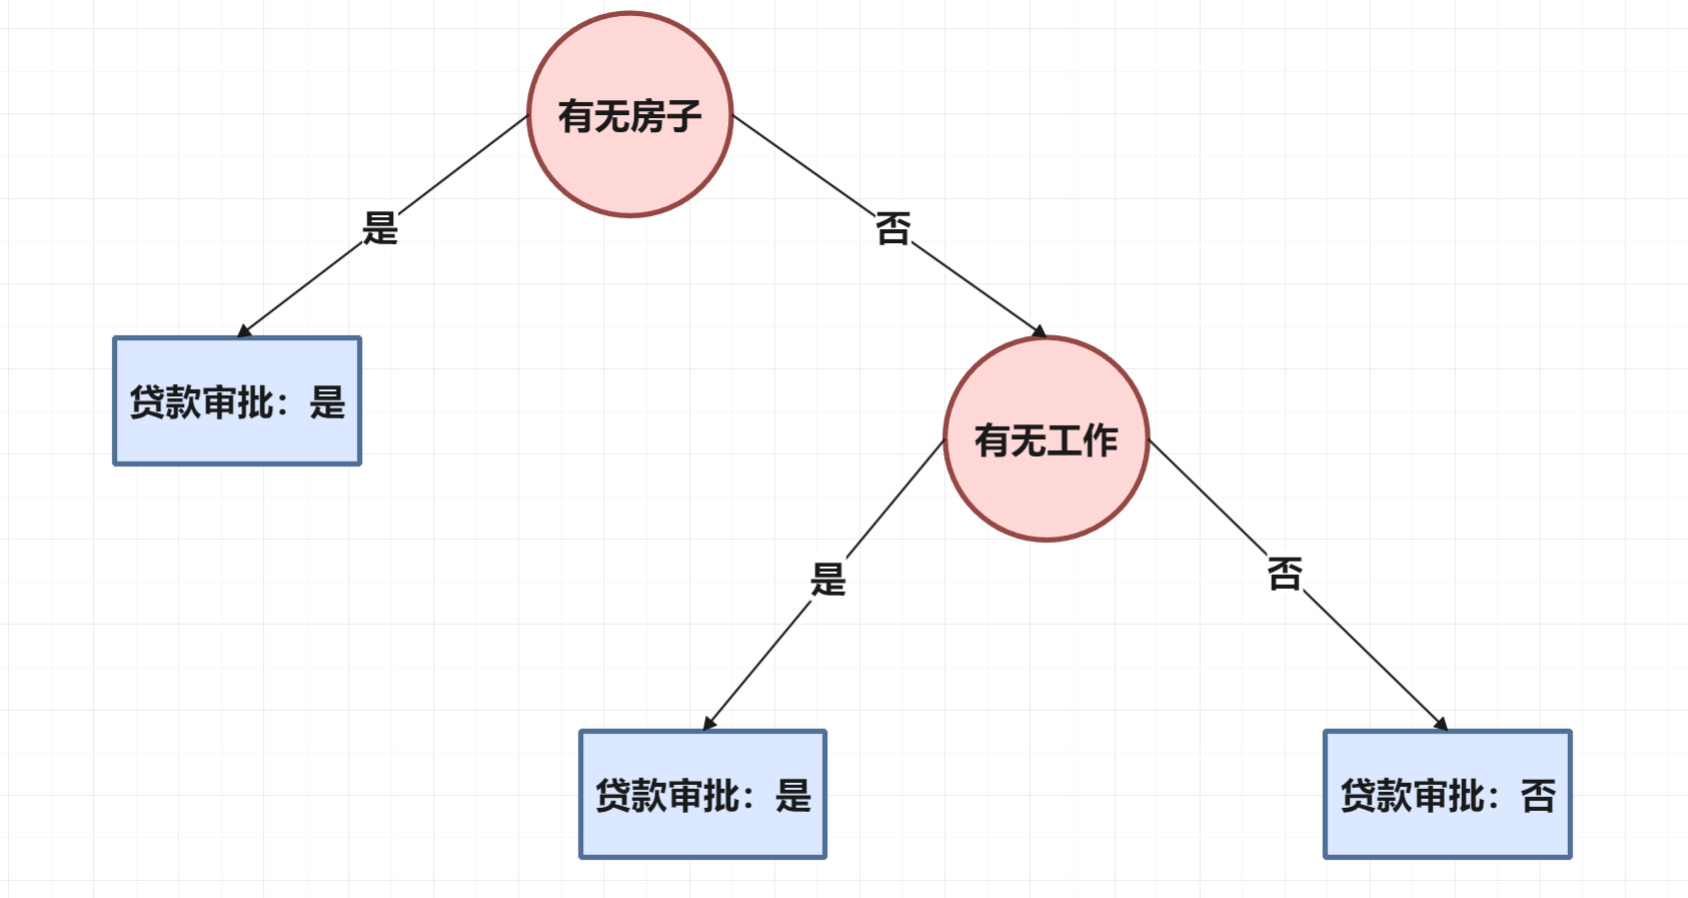
\includegraphics[width=0.35\linewidth]{image/决策树} 

}

\caption{决策树示意图}\label{fig:unnamed-chunk-17}
\end{figure}

\hypertarget{ux7b2cux4e09ux9898ux7528ux5e73ux65b9ux635fux5931ux51c6ux5219ux751fux6210ux4e00ux4e2aux4e8cux53c9ux56deux5f52ux6811}{%
\section{第三题:用平方损失准则生成一个二叉回归树}\label{ux7b2cux4e09ux9898ux7528ux5e73ux65b9ux635fux5931ux51c6ux5219ux751fux6210ux4e00ux4e2aux4e8cux53c9ux56deux5f52ux6811}}

\hypertarget{ux5bfcux5165ux6570ux636e-1}{%
\subsection{导入数据}\label{ux5bfcux5165ux6570ux636e-1}}

\begin{Shaded}
\begin{Highlighting}[]
\FunctionTok{library}\NormalTok{(readxl)}
\NormalTok{data }\OtherTok{\textless{}{-}} \FunctionTok{read\_excel}\NormalTok{(}\StringTok{"第三题数据.xlsx"}\NormalTok{, }\AttributeTok{col\_names =} \ConstantTok{FALSE}\NormalTok{)}
\NormalTok{data }\OtherTok{=} \FunctionTok{t}\NormalTok{(data)}
\FunctionTok{colnames}\NormalTok{(data) }\OtherTok{=} \FunctionTok{c}\NormalTok{(}\StringTok{\textquotesingle{}x\textquotesingle{}}\NormalTok{,}\StringTok{\textquotesingle{}y\textquotesingle{}}\NormalTok{)}
\NormalTok{data }\OtherTok{=} \FunctionTok{as.data.frame}\NormalTok{(data)}
\end{Highlighting}
\end{Shaded}

\hypertarget{ux8bbeux5b9aux505cux6b62ux8fedux4ee3ux7684ux51c6ux5219}{%
\subsection{设定停止迭代的准则}\label{ux8bbeux5b9aux505cux6b62ux8fedux4ee3ux7684ux51c6ux5219}}

若在某个节点\(R_m\)上,平方损失函数
\[L(R_m)=\sum_{i:\, x_i\in R_m}(y_i-\bar{y})^2 <\varepsilon\]
则停止对该节点的分裂。在本次实验中,我们设定\(\varepsilon=0.5\)

\begin{Shaded}
\begin{Highlighting}[]
\NormalTok{epsilon }\OtherTok{=} \FloatTok{0.5}
\end{Highlighting}
\end{Shaded}

\hypertarget{ux51c6ux5907ux5de5ux4f5cux7528ux4e8eux8ba1ux7b97ux5207ux5206ux70b9ux7684ux51fdux6570}{%
\subsection{准备工作:用于计算切分点的函数}\label{ux51c6ux5907ux5de5ux4f5cux7528ux4e8eux8ba1ux7b97ux5207ux5206ux70b9ux7684ux51fdux6570}}

\begin{Shaded}
\begin{Highlighting}[]
\NormalTok{split }\OtherTok{\textless{}{-}} \ControlFlowTok{function}\NormalTok{(data,i,j,epsilon)\{ }\CommentTok{\# i是左侧下标,j是右侧下标,epsilon是迭代停止界值}
  \ControlFlowTok{if}\NormalTok{(i}\SpecialCharTok{==}\NormalTok{j)\{ }\CommentTok{\# 如果数据集已经不可再分}
    \FunctionTok{return}\NormalTok{(}\ConstantTok{NULL}\NormalTok{)}
\NormalTok{  \}}
\NormalTok{  L }\OtherTok{=} \FunctionTok{sum}\NormalTok{((data[i}\SpecialCharTok{:}\NormalTok{j,]}\SpecialCharTok{$}\NormalTok{y}\SpecialCharTok{{-}}\FunctionTok{mean}\NormalTok{(data[i}\SpecialCharTok{:}\NormalTok{j,]}\SpecialCharTok{$}\NormalTok{y))}\SpecialCharTok{\^{}}\DecValTok{2}\NormalTok{)}
  \ControlFlowTok{if}\NormalTok{(L}\SpecialCharTok{\textless{}}\NormalTok{epsilon)\{ }\CommentTok{\# 如果数据集的损失函数已经足够小}
    \FunctionTok{return}\NormalTok{(}\ConstantTok{NULL}\NormalTok{)}
\NormalTok{  \}}
\NormalTok{  minL }\OtherTok{=} \ConstantTok{Inf}
\NormalTok{  minK }\OtherTok{=}\NormalTok{ i}
  \CommentTok{\# 寻找该子集的最佳切分点}
  \ControlFlowTok{for}\NormalTok{(k }\ControlFlowTok{in} \FunctionTok{seq}\NormalTok{(i,j}\DecValTok{{-}1}\NormalTok{))\{}
    \CommentTok{\# 切分,得到两个子集}
\NormalTok{    sub1 }\OtherTok{=}\NormalTok{ data[i}\SpecialCharTok{:}\NormalTok{k,]}
\NormalTok{    sub2 }\OtherTok{=}\NormalTok{ data[(k}\SpecialCharTok{+}\DecValTok{1}\NormalTok{)}\SpecialCharTok{:}\NormalTok{j,]}
    \CommentTok{\# 计算平方损失函数L}
\NormalTok{    L }\OtherTok{=} \FunctionTok{sum}\NormalTok{((sub1}\SpecialCharTok{$}\NormalTok{y}\SpecialCharTok{{-}}\FunctionTok{mean}\NormalTok{(sub1}\SpecialCharTok{$}\NormalTok{y))}\SpecialCharTok{\^{}}\DecValTok{2}\NormalTok{) }\SpecialCharTok{+} \FunctionTok{sum}\NormalTok{((sub2}\SpecialCharTok{$}\NormalTok{y}\SpecialCharTok{{-}}\FunctionTok{mean}\NormalTok{(sub2}\SpecialCharTok{$}\NormalTok{y))}\SpecialCharTok{\^{}}\DecValTok{2}\NormalTok{) }
    \ControlFlowTok{if}\NormalTok{( L}\SpecialCharTok{\textless{}}\NormalTok{minL )\{}
\NormalTok{      minL }\OtherTok{=}\NormalTok{ L}
\NormalTok{      minK }\OtherTok{=}\NormalTok{ k}
\NormalTok{    \}}
\NormalTok{  \}}
  \FunctionTok{return}\NormalTok{(minK) }\CommentTok{\# 返回最优的切分点}
\NormalTok{\}}
\end{Highlighting}
\end{Shaded}

\hypertarget{ux7b2cux4e00ux6b21ux5207ux5206}{%
\subsection{第一次切分}\label{ux7b2cux4e00ux6b21ux5207ux5206}}

\begin{Shaded}
\begin{Highlighting}[]
\CommentTok{\# 第一层的分界点}
\NormalTok{k}\FloatTok{.1} \OtherTok{=} \FunctionTok{split}\NormalTok{(data,}\DecValTok{1}\NormalTok{,}\DecValTok{10}\NormalTok{,epsilon)}
\FunctionTok{print}\NormalTok{(k}\FloatTok{.1}\NormalTok{) }\CommentTok{\# 5}
\end{Highlighting}
\end{Shaded}

\begin{verbatim}
## [1] 5
\end{verbatim}

将数据集按照\(x\le5\) 和
\(x>5\)拆成两个部分,可以使平方损失最小。对这两个部分继续进行分裂。

\hypertarget{ux7b2cux4e8cux6b21ux5207ux5206ux8fedux4ee3ux505cux6b62}{%
\subsection{第二次切分,迭代停止}\label{ux7b2cux4e8cux6b21ux5207ux5206ux8fedux4ee3ux505cux6b62}}

\begin{Shaded}
\begin{Highlighting}[]
\CommentTok{\# 第二层的分界点}
\NormalTok{k.}\FloatTok{2.1} \OtherTok{=} \FunctionTok{split}\NormalTok{(data,}\DecValTok{1}\NormalTok{,}\DecValTok{5}\NormalTok{,epsilon)}
\NormalTok{k.}\FloatTok{2.2} \OtherTok{=} \FunctionTok{split}\NormalTok{(data,}\DecValTok{6}\NormalTok{,}\DecValTok{10}\NormalTok{,epsilon)}
\FunctionTok{print}\NormalTok{(}\FunctionTok{c}\NormalTok{(k.}\FloatTok{2.1}\NormalTok{,k.}\FloatTok{2.2}\NormalTok{)) }\CommentTok{\# 3,7}
\end{Highlighting}
\end{Shaded}

\begin{verbatim}
## [1] 3 7
\end{verbatim}

将第一个部分又按照\(1\le x \le 3\)和\(3<x\le 5\)拆成两个子节点;将第二个部分按照\(5< x \le 7\)和\(7<x \le 10\)再拆成两个节点。

下面,尝试对第三层节点再次拆分

\begin{Shaded}
\begin{Highlighting}[]
\CommentTok{\# 第三层的分界点}
\NormalTok{k.}\FloatTok{3.1} \OtherTok{=} \FunctionTok{split}\NormalTok{(data,}\DecValTok{1}\NormalTok{,}\DecValTok{3}\NormalTok{,epsilon)}
\NormalTok{k.}\FloatTok{3.2} \OtherTok{=} \FunctionTok{split}\NormalTok{(data,}\DecValTok{4}\NormalTok{,}\DecValTok{5}\NormalTok{,epsilon)}
\NormalTok{k.}\FloatTok{3.3} \OtherTok{=} \FunctionTok{split}\NormalTok{(data,}\DecValTok{6}\NormalTok{,}\DecValTok{7}\NormalTok{,epsilon)}
\NormalTok{k.}\FloatTok{3.4} \OtherTok{=} \FunctionTok{split}\NormalTok{(data,}\DecValTok{8}\NormalTok{,}\DecValTok{10}\NormalTok{,epsilon)}
\FunctionTok{print}\NormalTok{(}\FunctionTok{c}\NormalTok{(k.}\FloatTok{3.1}\NormalTok{,k.}\FloatTok{3.2}\NormalTok{,k.}\FloatTok{3.3}\NormalTok{,k.}\FloatTok{3.4}\NormalTok{)) }\CommentTok{\# 全都是NULL}
\end{Highlighting}
\end{Shaded}

\begin{verbatim}
## NULL
\end{verbatim}

发现第三层每个叶子节点的损失函数都小于临界值\(\varepsilon\),不需要继续拆分,则停止迭代。

\hypertarget{ux6bcfux4e2aux5212ux5206ux7684ux9884ux6d4bux503c}{%
\subsection{每个划分的预测值}\label{ux6bcfux4e2aux5212ux5206ux7684ux9884ux6d4bux503c}}

每个划分的输出值为该划分中所有样本的平均值,那么,上述四个类别的划分的输出值分别为:

\begin{Shaded}
\begin{Highlighting}[]
\NormalTok{c1 }\OtherTok{=} \FunctionTok{mean}\NormalTok{(data}\SpecialCharTok{$}\NormalTok{y[}\DecValTok{1}\SpecialCharTok{:}\DecValTok{3}\NormalTok{])}
\NormalTok{c2 }\OtherTok{=} \FunctionTok{mean}\NormalTok{(data}\SpecialCharTok{$}\NormalTok{y[}\DecValTok{4}\SpecialCharTok{:}\DecValTok{5}\NormalTok{])}
\NormalTok{c3 }\OtherTok{=} \FunctionTok{mean}\NormalTok{(data}\SpecialCharTok{$}\NormalTok{y[}\DecValTok{6}\SpecialCharTok{:}\DecValTok{7}\NormalTok{])}
\NormalTok{c4 }\OtherTok{=} \FunctionTok{mean}\NormalTok{(data}\SpecialCharTok{$}\NormalTok{y[}\DecValTok{8}\SpecialCharTok{:}\DecValTok{10}\NormalTok{])}
\FunctionTok{print}\NormalTok{(}\FunctionTok{rbind}\NormalTok{(}\FunctionTok{c}\NormalTok{(}\StringTok{\textquotesingle{}c1\textquotesingle{}}\NormalTok{,}\StringTok{\textquotesingle{}c2\textquotesingle{}}\NormalTok{,}\StringTok{\textquotesingle{}c3\textquotesingle{}}\NormalTok{,}\StringTok{\textquotesingle{}c4\textquotesingle{}}\NormalTok{),}\FunctionTok{c}\NormalTok{(c1,c2,c3,c4)))}
\end{Highlighting}
\end{Shaded}

\begin{verbatim}
##      [,1]   [,2]   [,3]    [,4]              
## [1,] "c1"   "c2"   "c3"    "c4"              
## [2,] "4.72" "5.57" "7.475" "8.64333333333333"
\end{verbatim}

\hypertarget{ux4e8cux53c9ux56deux5f52ux6811ux793aux610fux56fe}{%
\subsection{二叉回归树示意图}\label{ux4e8cux53c9ux56deux5f52ux6811ux793aux610fux56fe}}

\begin{Shaded}
\begin{Highlighting}[]
\NormalTok{ knitr}\SpecialCharTok{::}\FunctionTok{include\_graphics}\NormalTok{(}\StringTok{"image/回归树.png"}\NormalTok{)}
\end{Highlighting}
\end{Shaded}

\begin{figure}

{\centering 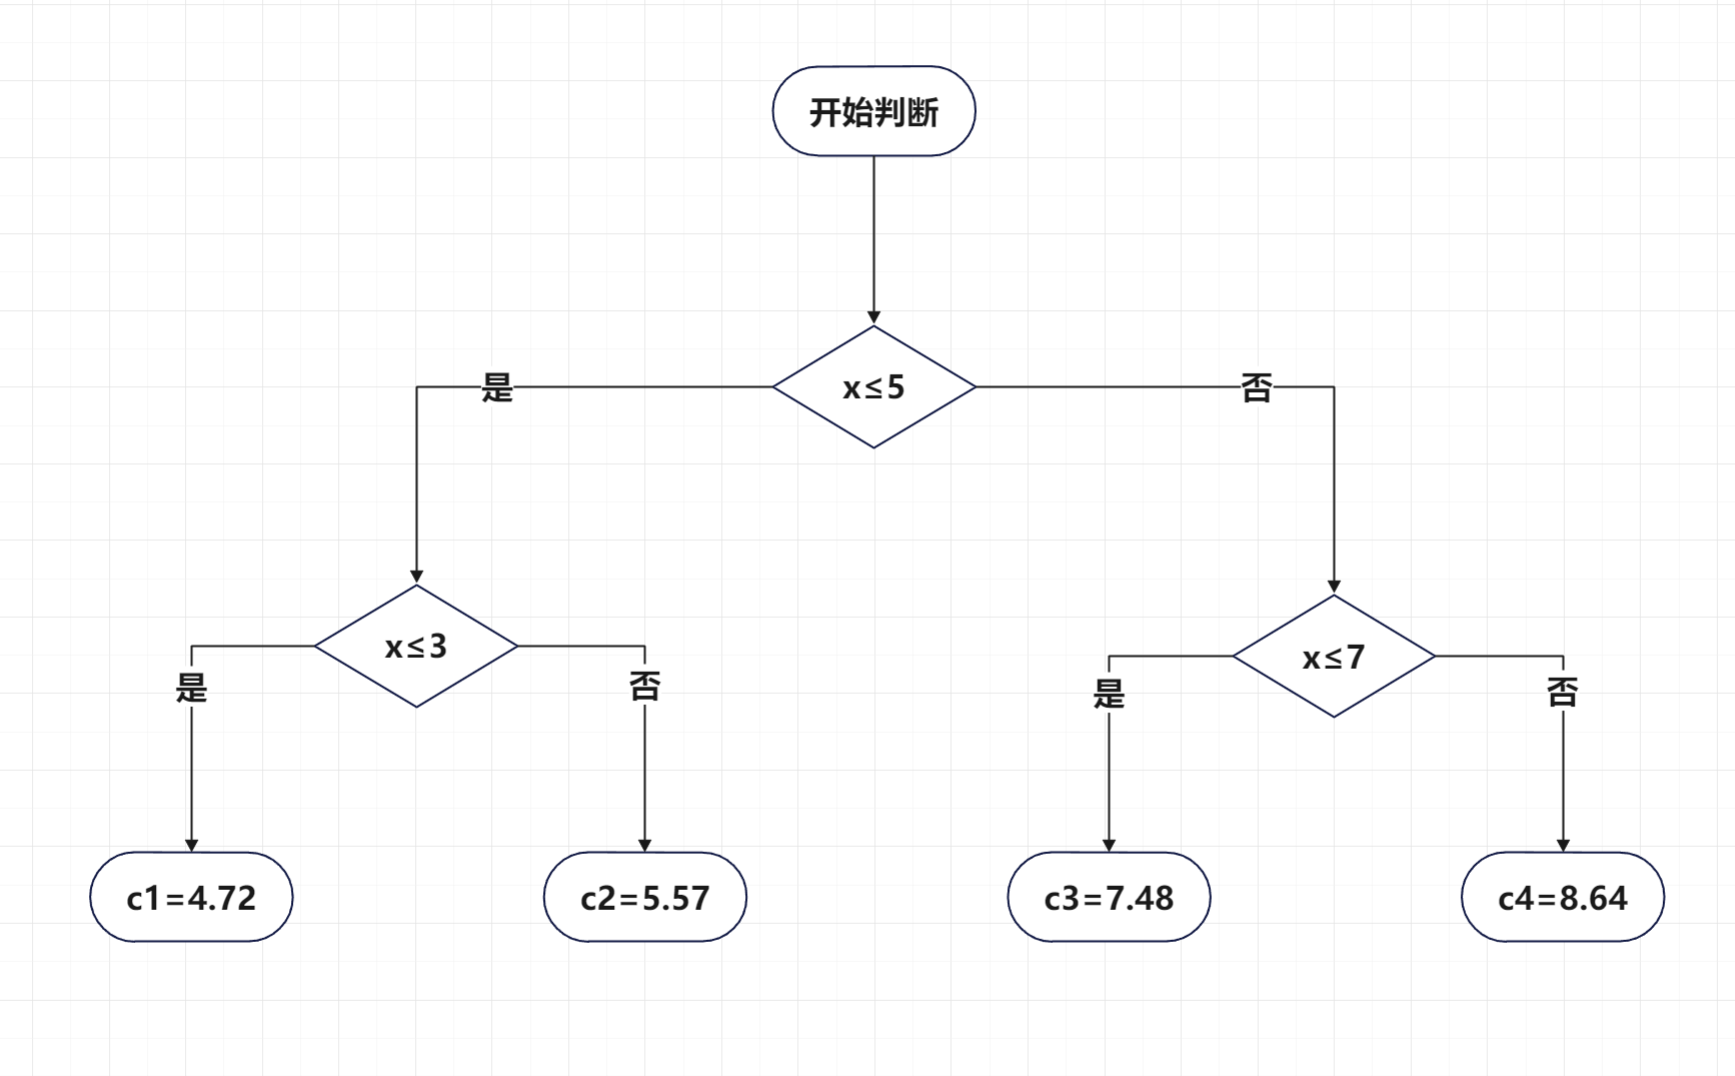
\includegraphics[width=0.5\linewidth]{image/回归树} 

}

\caption{回归树示意图}\label{fig:unnamed-chunk-25}
\end{figure}

\hypertarget{ux7b2cux56dbux9898ux8bc1ux660ecartux526aux679dux8fc7ux7a0bux4e2dalpha_kux5355ux8c03ux9012ux589e}{%
\section{\texorpdfstring{第四题:证明Cart剪枝过程中\(\alpha_k\)单调递增}{第四题:证明Cart剪枝过程中\textbackslash alpha\_k单调递增}}\label{ux7b2cux56dbux9898ux8bc1ux660ecartux526aux679dux8fc7ux7a0bux4e2dalpha_kux5355ux8c03ux9012ux589e}}

\hypertarget{ux7b2ckux6b65ux7684ux60c5ux51b5}{%
\subsection{\texorpdfstring{第\(k\)步的情况}{第k步的情况}}\label{ux7b2ckux6b65ux7684ux60c5ux51b5}}

在第\(k\)步中,设 \[
\alpha_k = \mathop{\min}_{t\,\in \,\mathcal{M}_k} g_k(t) = g_k(a)
\] 其中 \[
g_k(t) = \frac{C(t)-C(T_t)}{|T_t|-1}
\]

\(C(t)\)表示以节点\(t\)为单节点的预测误差,\(C(t)\)不随以\(t\)为根节点的子树的剪枝而发生变化。\(C(T_t)=\sum_{\tau \in T_t} N_\tau H_\tau\),其中\(\tau\)是以\(t\)为根节点的子树的叶节点,\(N_\tau\)是叶节点\(\tau\)的样本数,\(H_\tau\)是\(\tau\)节点的熵。\(|T_t|\)是以\(t\)为根节点的子树的所有叶子节点的个数。

注意到在第\(k\)步中,\(\alpha_k = \frac{C(a)-C(T_a)}{|T_a|-1}\),且由于满足剪枝条件的节点是唯一的,则对于任意不为\(a\)的内部节点\(t\),都成立\(g_k(t)>\alpha_k,\,t\ne a\).

\hypertarget{ux7b2ck1ux6b65ux7684ux60c5ux51b5}{%
\subsection{\texorpdfstring{第\(k+1\)步的情况}{第k+1步的情况}}\label{ux7b2ck1ux6b65ux7684ux60c5ux51b5}}

剪枝后,对于\(\forall t \in \mathcal{M}_{k+1}\),若\(t\)不是\(a\)的祖先节点,也即以\(t\)为根节点的子树不包含\(a\),则仍然有\(g_{k+1}(t) = g_k(t)>\alpha_k\).

若\(t\)是\(a\)的祖先节点,则以\(t\)为根节点的子树的预测误差增加了\(C(a)-C(T_a)\),叶子节点数量减少了\(|T_a|-1\)。我们可以得到:

\begin{align*}
g_{k+1}(t) &= \frac{C^{(k+1)} (t) - C^{(k+1)}(T_t)}{|T_t^{(k+1)}|-1} \\
&= \frac{C(t) - C(T_t) - [ C(a)-C(T_a)]}{|T_t|-1 - (|T_a|-1)}\\
\end{align*}

由于 \[
g_k(t) = \frac{C(t)-C(T_t)}{|T_t|-1} > \alpha_k
\]

并且 \begin{align*}
 \quad C(a)-C(T_a) = \alpha_k \,\left(|T_a|-1\right) 
\end{align*}

则有如下等价关系: \begin{align*}
 &\quad \frac{C(t) - C(T_t) - [ C(a)-C(T_a)]}{|T_t|-1 - (|T_a|-1)} > \alpha_k \\
 &\Leftrightarrow  C(t) - C(T_t) - [ C(a)-C(T_a)] > \alpha_k [|T_t|-1 -(|T_a|-1)] \\
 & \Leftrightarrow   C(t) - C(T_t) > \alpha_k (|T_t|-1) \\
 & \Leftrightarrow \frac{C(t)-C(T_t)}{|T_t|-1} > \alpha_k
\end{align*}

在第\(k+1\)步时,\(\forall t \in \mathcal{M}_{k+1},\,g_{k+1}(t)>\alpha_k\),因此,也有

\begin{equation*}
\alpha_{k+1}= \min_{t  \in  \mathcal{M}_{k+1}}g_{k+1}(t) > \alpha_k 
\end{equation*}

证毕

\end{document}
